\documentclass[journal]{IEEEtran}

\usepackage{amsmath,amssymb}
\usepackage{newtxtext,newtxmath}
\usepackage{graphicx}
\usepackage{booktabs}
\usepackage{multirow}
\usepackage{array}
\usepackage{cite}
\usepackage{url}
\usepackage{xcolor}
\usepackage{microtype}
\usepackage{placeins}
\usepackage{balance}
\usepackage[hidelinks,unicode]{hyperref}
\hypersetup{pdftitle={Evaluating Focus--Diffusion Feature Fusion for Data-Limited Pedestrian Detection},pdfauthor={Jiaxu Chen}}

\graphicspath{{figures/}}
\newcommand{\mapfifty}{mAP$_{50}$}
\newcommand{\mapcoco}{mAP$_{50:95}$}
\newcommand{\method}{FDPN}
\newcommand{\projectrepository}{\url{https://github.com/shen982/RTDETR-R18-FDPN-Pedestrian-Detection}}

\title{Evaluating Focus--Diffusion Feature Fusion\\for Data-Limited Pedestrian Detection}

\author{Jiaxu Chen\\[0.35em]
{\normalfont\small Department of Automation, North China Electric Power University}\\[-0.1em]
{\normalfont\small Baoding, China}\\[-0.1em]
{\normalfont\small E-mail: \href{mailto:17736460722@163.com}{17736460722@163.com}}}

\begin{document}
\raggedbottom
\maketitle

\begin{abstract}
With limited pedestrian annotations, cross-scale fusion must reconcile spatial detail and semantic context, yet the benefit of increasing fusion capacity and repeating aggregation remains uncertain. We examine an existing Focusing Diffusion Pyramid Network (FDPN) configuration within RT-DETR-R18. Its neck aligns three feature levels, aggregates spatial context with parallel depthwise kernels, and redistributes the representation across detector scales. Under matched training protocols, we compare this configuration with the original fusion path and a near-parameter-matched widened-neck control, then assess component sensitivity. On Penn--Fudan, three-seed mean AP over IoU thresholds 0.50--0.95 improves by 1.22 and 0.86 percentage points over the two controls, respectively. Mean AP at IoU 0.50 falls by 1.42 points, while inference parameters increase by 11.9\%. Exploratory 100-epoch comparisons on fixed VOC2007-person and COCO2017-person subsets yield AP gains of 0.56 and 1.19 points. A single-seed ablation favors the complete multi-kernel configuration over a single $5\times5$ kernel. Refocusing yields no observed gain in AP over IoU 0.50--0.95, but improves AP at IoU 0.50. Thus, the observed benefit depends on the metric and evaluation setting; the ablation motivates, but does not establish the superiority of, a simpler fusion path.
\end{abstract}

\begin{IEEEkeywords}
pedestrian detection, end-to-end object detection, cross-scale feature fusion, multi-kernel context modeling, data-limited learning
\end{IEEEkeywords}

\section{Introduction}
Object detection estimates object categories and spatial extents. Detection Transformer (DETR) formulates this task as set prediction through object queries and bipartite assignment, avoiding the duplicate-removal stage used in many conventional detectors \cite{carion2020detr,vaswani2017attention}. Subsequent work improves multi-scale interaction and optimization through sparse attention, spatial queries, and denoising \cite{zhu2021deformable,liu2022dab,zhang2023dino}. RT-DETR combines efficient within-scale attention with convolutional cross-scale fusion and informative query selection, providing a compact R18 baseline in which the feature neck can be studied without replacing the complete detector \cite{zhao2024rtdetr}.

Pedestrian detection under limited annotations requires the fusion path to preserve fine spatial cues while incorporating semantic context. Neighbor-wise pyramids exchange information across successive resolutions \cite{lin2017fpn,liu2018panet}; direct multi-level aggregation instead aligns distant levels before contextualization. The latter offers a shorter cross-scale path, but a larger fusion neck can also improve accuracy simply by adding capacity or computation. It is therefore unclear whether the existing focus--diffusion configuration benefits this detector beyond a widened conventional neck, and whether its second focusing stage is necessary. Here, \emph{data-limited} means fully supervised learning from small annotated partitions, not a formal few-shot protocol.

\begin{figure*}[t]
    \centering
    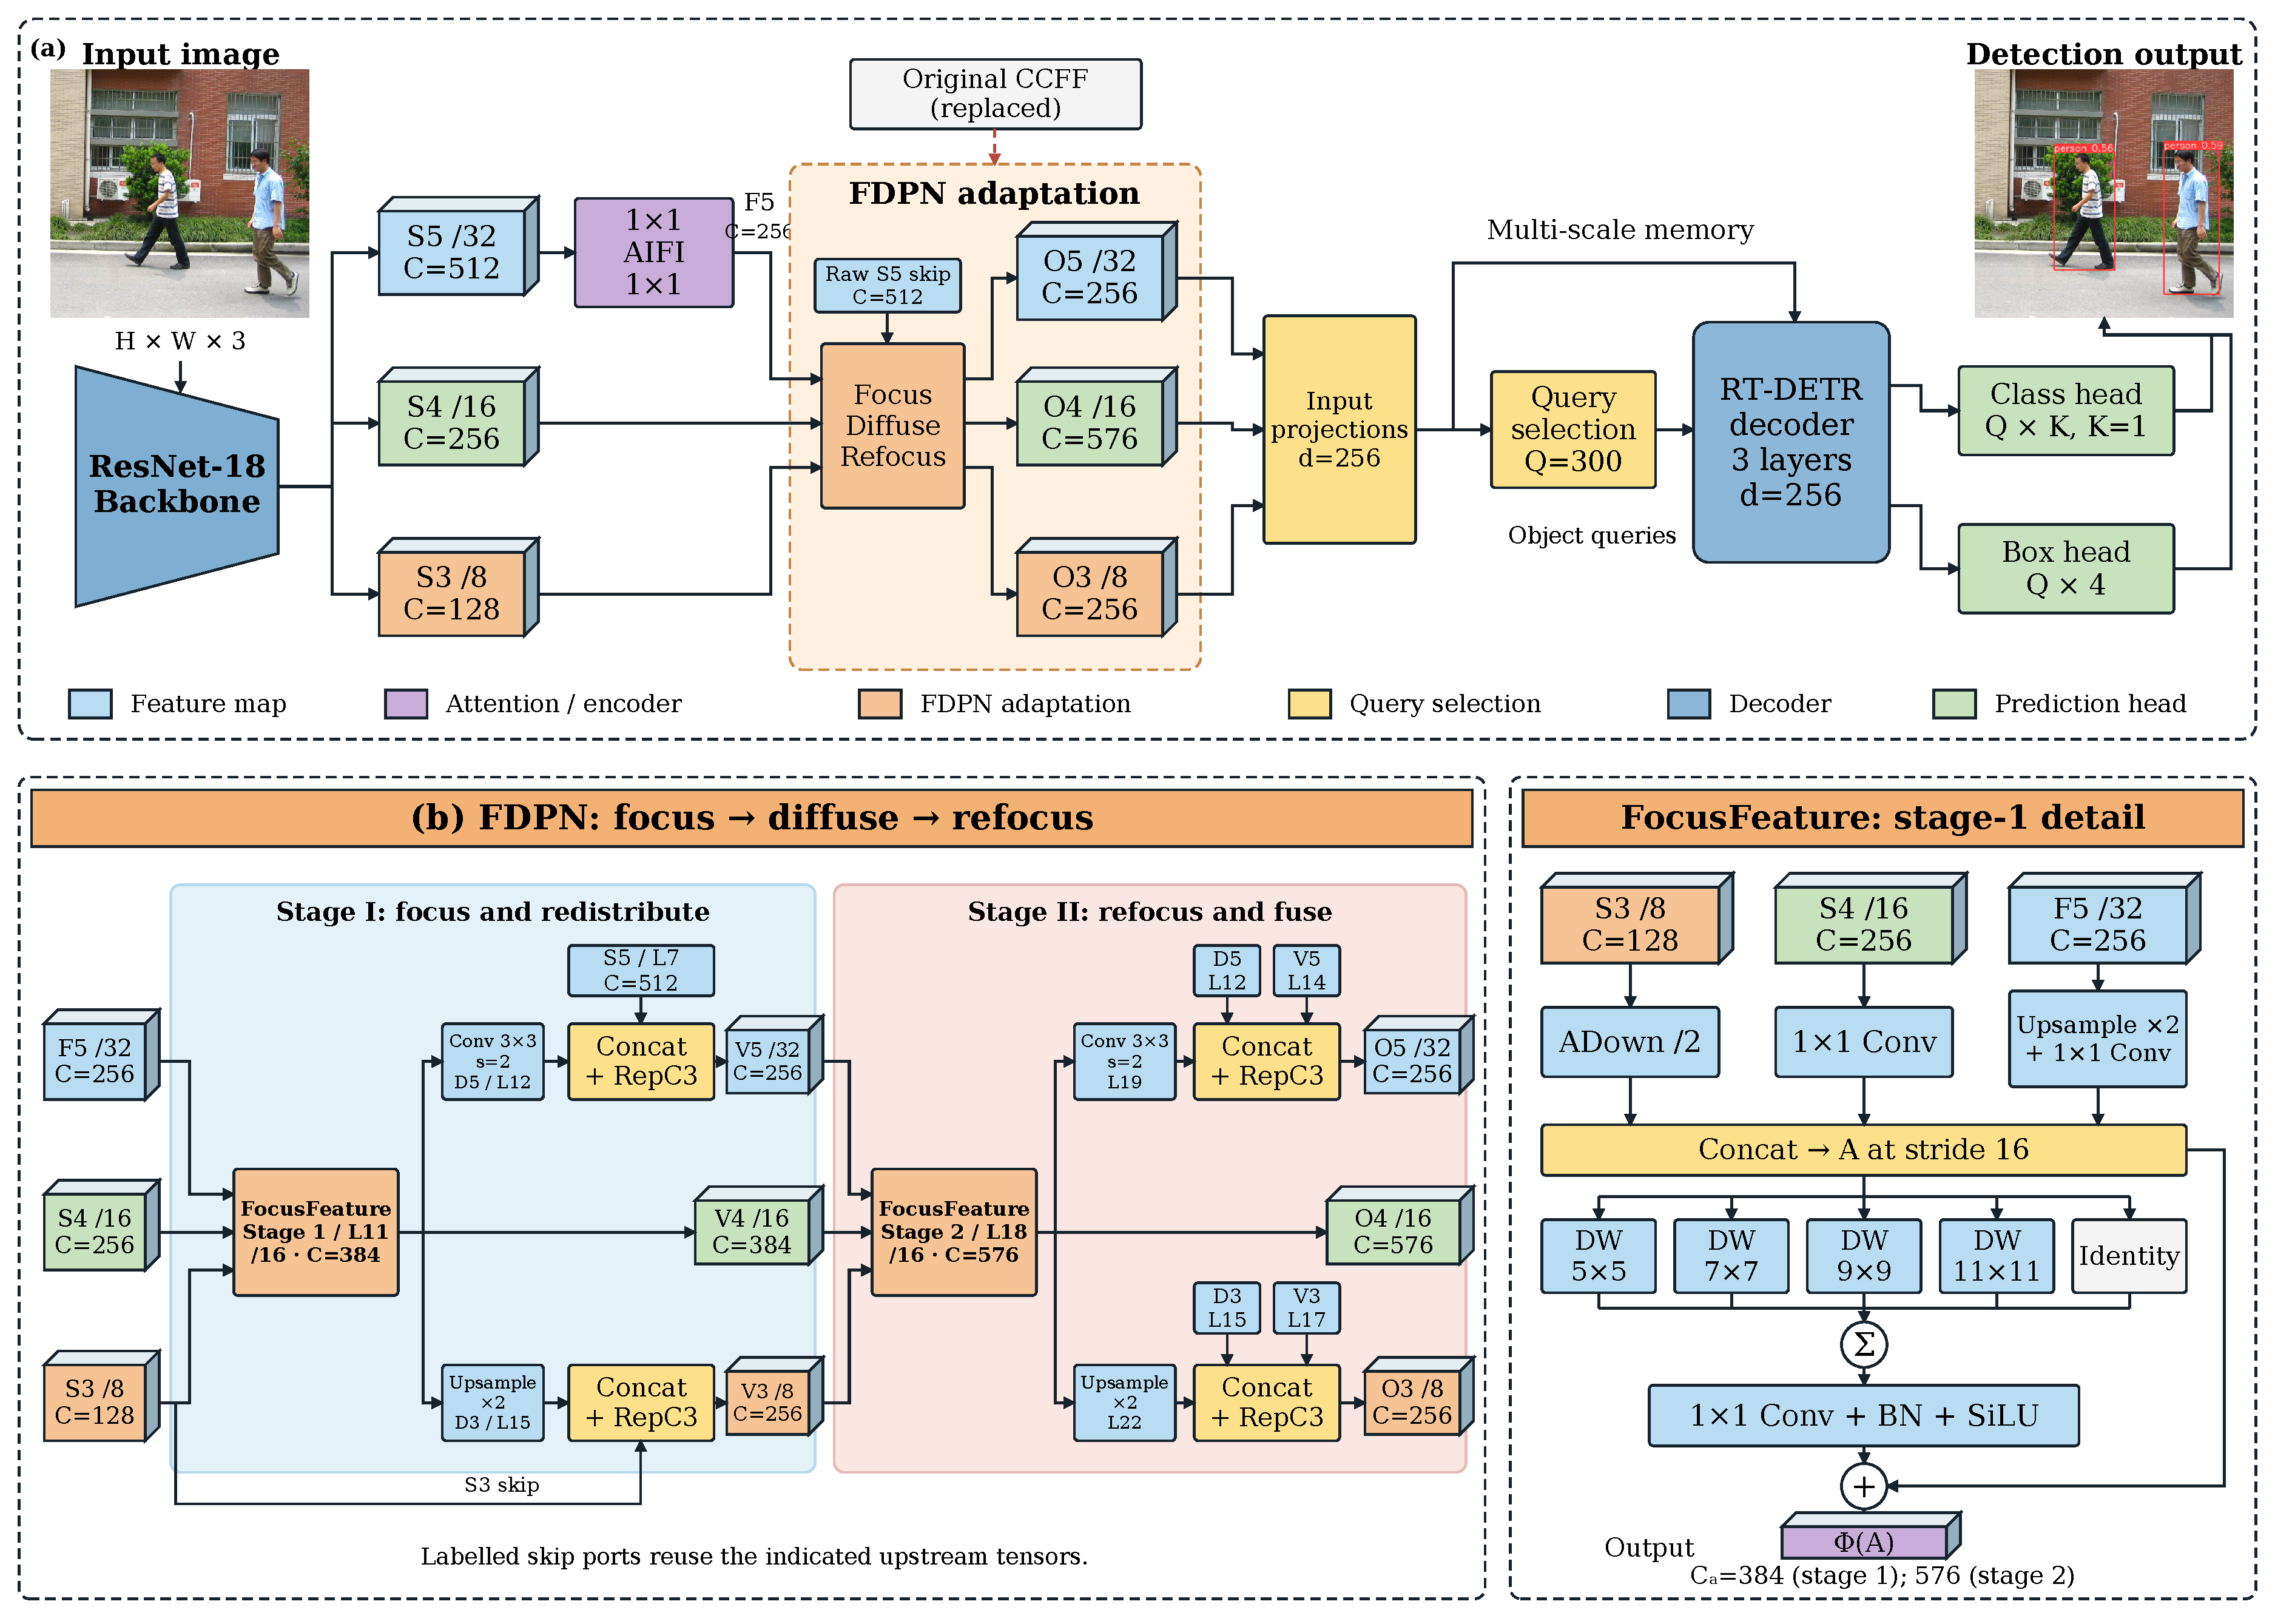
\includegraphics[width=\textwidth]{architecture_visio_revision.pdf}
    \caption{Code-aligned FDPN adaptation of RT-DETR-R18. (a) Detector overview with CCFF replaced by FDPN. (b) Two focusing stages, redistribution paths, labelled skip ports, and first-stage FocusFeature detail (right). $S_i$ and $V_i$ correspond to backbone $P_i$ and intermediate $Z_i^{(1)}$ in Section~III. Insets show held-out Penn--Fudan image FudanPed00001 and its FDPN predictions with display threshold 0.50. The diagram is redrawn from the implemented graph, following RT-DETR~\cite{zhao2024rtdetr} and the attributed focus--diffusion design~\cite{luo2026fdfpn}; integration details are summarized in Appendix~B.}
    \label{fig:overview}
\end{figure*}

We study an FDPN-equipped RT-DETR-R18 graph already present in the attributed source bundle \cite{modulebundle2026}, informed by published focus--diffusion work \cite{luo2026fdfpn}. It replaces convolutional cross-scale feature fusion (CCFF) with direct three-level alignment, parallel depthwise kernels, bidirectional redistribution, and a second learned aggregation. The backbone, attention-based intra-scale feature interaction (AIFI), query-selection mechanism, decoder architecture, and objective are retained; input projections accommodate the changed feature widths. This setting permits a controlled evaluation of the existing design, although its topology, feature width, and computational cost cannot be fully disentangled. Aggregate AP also cannot establish a specific benefit for small or occluded pedestrians.

This study makes two empirical contributions:
\begin{itemize}
    \item \emph{Performance and boundary assessment:} matched RT-DETR-R18 comparisons on Penn--Fudan and two person-only subsets, including three training seeds, a near-parameter-matched neck control, two budgets, and computational-cost analysis. These comparisons distinguish an improvement in cross-threshold AP from a decrease in AP at IoU 0.50.
    \item \emph{Component sensitivity:} source-aligned characterization and ablations of the supplied fusion graph. They favor the tested full multi-kernel configuration but show no additional gain in \mapcoco{} from repeated focusing, with a trade-off in \mapfifty{}. This identifies a candidate simplification rather than a proven optimal design.
\end{itemize}
The fusion topology itself is attributed to the supplied implementation, not claimed as a newly invented architecture.

\section{Related Work}
\subsection{Transformer-Based End-to-End Detection}
Transformer-based detectors formulate object detection as set prediction rather than dense proposal filtering. This research line combines global feature interaction, a fixed set of object queries, bipartite assignment, and parallel decoding to produce one-to-one predictions \cite{carion2020detr}. Subsequent studies have developed several complementary families of techniques: sparse multi-scale attention improves the efficiency of spatial interaction \cite{zhu2021deformable}; explicit spatial query representations strengthen positional reasoning \cite{liu2022dab}; and denoising, mixed query initialization, and iterative refinement stabilize optimization \cite{zhang2023dino}. These advances collectively establish a mature end-to-end detection framework in which feature encoding, query initialization, and set decoding can be studied as distinct components.

A parallel body of work investigates how to retain the end-to-end formulation under real-time constraints. Efficient designs reduce redundant interaction over multi-scale tokens, decouple within-scale attention from cross-scale convolutional fusion, and expose decoder depth as an accuracy--latency control \cite{zhao2024rtdetr}. This category of models is particularly suitable for controlled architectural study because the backbone, encoder, query selection, and decoder have clearly separated roles. The present work operates within this framework and modifies only the cross-scale feature path.

\subsection{Multi-Scale Representation Learning}
Multi-scale representation is a long-standing requirement in object detection. Pyramid-based studies construct semantically enriched high-resolution maps through top-down lateral fusion \cite{lin2017fpn}, add bottom-up paths to shorten information transfer \cite{liu2018panet}, or repeat bidirectional fusion with normalized learnable weights \cite{tan2020efficientdet}. Across these designs, the common objective is to reconcile the fine spatial structure of shallow features with the semantic abstraction of deep features while controlling the cost of resampling and fusion.

Existing research can be broadly grouped into neighbor-wise pyramids, weighted repeated pyramids, and direct multi-level aggregation. The first two groups propagate information mainly through adjacent resolutions; the third aligns several levels to a common spatial scale before joint processing. Collectively, this literature indicates that the topology and receptive field of the neck can influence detection independently of the backbone and prediction head. It also motivates examining whether direct three-level interaction is advantageous when supervision is limited and object scale varies substantially.

\subsection{Focus--Diffusion Feature Fusion}
Recent focus--diffusion studies instantiate direct multi-level aggregation through two operations. A focusing stage aligns shallow, intermediate, and deep features, then aggregates multiple receptive fields using depthwise convolution; a diffusion stage redistributes the context-enriched representation to the detection scales. Published FDFPN work combines these operations in a structured neck and reports their use in multi-scale detection \cite{luo2026fdfpn}. Related engineering implementations, including the supplied bundle used in this study, expose the same design as a reusable FocusFeature operator and an FDPN model graph \cite{modulebundle2026}.

The supplied implementation already includes an RT-DETR fusion graph. However, an available architecture does not establish its effect under limited pedestrian annotations: decoder interfaces, optimization schedules, and data regimes can alter the outcome of a neck substitution. This study therefore examines the conditional accuracy and component sensitivity of the existing configuration under matched evaluation protocols.

\section{Method}
\subsection{Problem Formulation and Baseline}
Let an input image $I$ have spatial size $H\times W$ and three channels. The ResNet-18-style backbone \cite{he2016resnet} produces $\{P_3,P_4,P_5\}$ at strides $\{8,16,32\}$ with channel widths $\{128,256,512\}$. We denote by $F_5$ the 256-channel output of the projection--AIFI--projection sequence (layers 8--10), reserving $P_5$ for the raw 512-channel backbone feature. In the baseline, CCFF propagates information along top-down and bottom-up paths to form three decoder inputs. The retained implementation selects the top $Q=300$ encoder positions by their maximum class score to initialize object queries; a three-layer RT-DETR decoder predicts class probabilities and normalized boxes.

Both configurations retain the same RT-DETR one-to-one assignment, classification and box-regression losses, query count, and decoder architecture \cite{carion2020detr,zhao2024rtdetr}. The experimental intervention is the fusion path and its required input projections, including the resulting change in model capacity.

\subsection{Overall Architecture}
Figure~\ref{fig:overview} situates the supplied configuration within RT-DETR; Appendix~B summarizes its interfaces. FDPN replaces CCFF while retaining the backbone, AIFI, query selection, and decoder architecture. The first FocusFeature block receives $(F_5,P_4,P_3)$, not the raw $P_5$. Its stride-16 representation is redistributed toward strides 32 and 8, concatenated with raw $P_5$ and $P_3$, respectively, and refined by RepC3 blocks. A second FocusFeature block reaggregates the three streams at stride 16. Final bidirectional fusion produces the decoder inputs.

The two focusing stages share an operator structure but have independent parameters; refocusing therefore denotes a second learned aggregation, not recurrent weight sharing. Appendix~B records the exact layer interfaces.

The resulting decoder-input widths are $\{256,576,256\}$, compared with $\{256,256,256\}$ in the baseline. The decoder input projections adapt to these widths; its hidden dimension, depth, and query count are unchanged. Consequently, the neck substitution also changes capacity, and is not an equal-width or equal-parameter comparison.

\subsection{Resolution-Aligned Cross-Scale Aggregation}
The first FocusFeature block aligns three resolutions at $P_4$. The $F_5$ branch is upsampled by a factor of two and projected with a $1\times1$ convolution; the $P_4$ branch is projected directly; and the $P_3$ branch is reduced with ADown. ADown first applies average pooling, splits the channels, and processes the two halves with stride-2 convolution and max-pooling-plus-projection paths before concatenation. Let $U$, $M$, and $D$ denote these transforms. The aligned tensor is
\begin{equation}
A=\operatorname{Concat}\bigl(U(F_5),M(P_4),D(P_3)\bigr).
\label{eq:align}
\end{equation}
Each branch is projected to half of the middle-level input width; hence the concatenated tensor has $1.5$ times that width. This bounded expansion preserves information from all three levels without applying dense large-kernel convolution over a full-width concatenation.

\subsection{Parallel Multi-Kernel Context Modeling}
The aligned tensor is contextualized by parallel depthwise convolutions with kernel sizes $\mathcal{K}=\{5,7,9,11\}$. Let $\mathrm{DW}_k$ denote a depthwise convolution and $\mathcal{P}$ the pointwise convolution followed by batch normalization and SiLU activation. A generic focusing stage computes
\begin{equation}
\Phi(A)=A+\mathcal{P}\!\left(A+\sum_{k\in\mathcal{K}}\mathrm{DW}_k(A)\right).
\label{eq:focus}
\end{equation}
The inner identity branch preserves the aligned representation, while the outer residual provides a direct feature and gradient path. Depthwise filtering supplies multiple receptive-field extents without the channel-quadratic cost of dense spatial convolution; channel mixing is performed by $\mathcal{P}$. The kernel set is fixed rather than input-adaptive. We denote the independently parameterized first and second stages by $\Phi_1$ and $\Phi_2$.

\subsection{Bidirectional Redistribution and Refocusing}
Here, diffusion denotes deterministic cross-scale feature redistribution, not a stochastic generative process. Let $Z_4^{(1)}=\Phi_1(A)$ be the first focused representation. Its stride-2 convolution and upsampling branches are denoted by $D_5$ (layer 12) and $U_3$ (layer 15). Concatenating these with raw $P_5$ and $P_3$, respectively, followed by RepC3 yields $Z_5^{(1)}$ and $Z_3^{(1)}$. The intermediate representation and the redistributed streams are then refocused:
\begin{equation}
Z_4^{(2)}=\Phi_2\!\left(\operatorname{Align}
\bigl(Z_5^{(1)},Z_4^{(1)},Z_3^{(1)}\bigr)\right).
\end{equation}
A final stride-2 branch from $Z_4^{(2)}$ is concatenated with both $D_5$ and $Z_5^{(1)}$; the upsampling branch is concatenated with both $U_3$ and $Z_3^{(1)}$. RepC3 refines the two three-input concatenations into $O_5$ and $O_3$, while $O_4=Z_4^{(2)}$. Thus, the final outputs retain the direct first-stage redistribution paths as well as the refined streams. The hypothesis is that direct multi-level interaction and broad contextual aggregation benefit pedestrian detection under limited annotations. Section~IV examines the complete configuration and the sensitivity to repeated focusing separately.

\section{Experiments}
We evaluate whether the existing fusion configuration improves detection beyond a widened conventional neck, how its effect varies with data and optimization budget, and whether both aggregation stages are supported by component evidence.

\begin{figure*}[t]
    \centering
    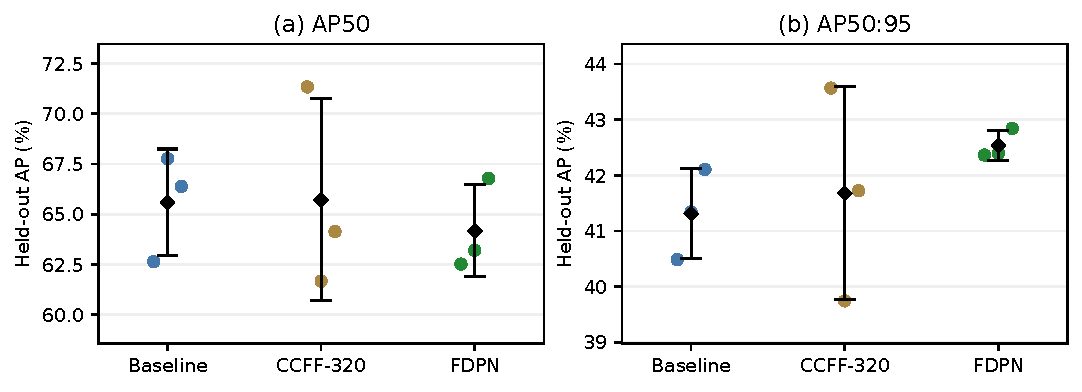
\includegraphics[width=0.92\textwidth]{robustness_summary.pdf}
    \caption{Principal Penn--Fudan comparison across three training seeds (30 epochs). Points show individual held-out runs; diamonds and error bars show means $\pm$ sample standard deviations, not confidence intervals. (a) AP at IoU 0.50; (b) AP averaged over IoU 0.50--0.95. The fixed 25-image test partition is reused across seeds.}
    \label{fig:seed_results}
\end{figure*}

\subsection{Experimental Settings}
\emph{Datasets.} The primary benchmark is Penn--Fudan \cite{wang2007recognition}, complemented by fixed person-only subsets of VOC2007 \cite{everingham2010voc,voc2007official} and COCO2017 \cite{lin2014coco,coco2017official}. Penn--Fudan boxes are derived from the official instance masks; the 423 instances agree with the archive's text annotations. Table~\ref{tab:public_splits} summarizes the image-disjoint partitions. VOC samples the official training, validation, and test pools; COCO uses disjoint train2017 samples for training/validation and val2017 samples for testing. Each public partition contains 20\% person-free images; images containing difficult persons in VOC or crowd persons in COCO are excluded because the evaluator does not implement the corresponding ignore conventions. All person boxes in eligible images are retained. Models are retrained independently on each dataset. These sampled single-class evaluations are neither full official benchmark results nor zero-shot transfer tests.

\begin{table}[t]
\centering
\caption{Evaluation partitions: image/person-instance counts.}
\label{tab:public_splits}
\setlength{\tabcolsep}{4pt}
\begin{tabular}{lrrr}
\toprule
Dataset & Train & Val & Test\\
\midrule
Penn--Fudan & 120/294 & 25/65 & 25/64\\
VOC-person & 300/482 & 50/77 & 100/152\\
COCO-person & 300/748 & 50/121 & 100/297\\
\bottomrule
\end{tabular}
\end{table}


\emph{Training protocol.} Both architectures are trained from scratch with identical data and optimization settings within each comparison \cite{ultralytics2023,paszke2019pytorch}. Training uses $416\times416$ inputs, batch size 4, AdamW \cite{loshchilov2019adamw}, and learning rate and weight decay of $10^{-4}$ on an RTX 3090. The initial Penn--Fudan comparison and component ablations use 30 epochs and seed 2026; public-subset comparisons use independent 30- and 100-epoch runs. A later Penn--Fudan follow-up trains the baseline, FDPN, and a widened CCFF control afresh with seeds 2026, 2027, and 2028, also for 30 epochs. All nine follow-up training runs finish before their held-out evaluations. The previously used partition is retained, so this is a seed-sensitivity study, not a fresh independent test. Appendix~A summarizes this evaluation.

\emph{Evaluation.} The primary metric is COCO-style \mapcoco{}, averaged over intersection-over-union (IoU) thresholds 0.50:0.05:0.95; \mapfifty{}, precision, and recall provide complementary summaries. With one foreground class, mAP equals person-class AP. For every model, the selected checkpoint is the best within the declared training budget according to validation fitness, $0.1\,\mathrm{AP}_{50}+0.9\,\mathrm{AP}_{50:95}$. All held-out metrics for a run are computed from that same checkpoint; epochs are not selected by test-set improvement or separately for different metrics. Precision and recall use toolkit-selected F1 operating points rather than a shared deployment threshold. AP is reported in percent; all differences are computed from unrounded values and expressed in percentage points.

\subsection{Detection Accuracy Across Data Sources}
Table~\ref{tab:robustness} provides the principal repeated-run comparison on Penn--Fudan. The widened CCFF-320 control is selected by parameter proximity before training: its 22.029 M inference parameters differ from FDPN's 22.236 M by 0.93\%. It retains the baseline fusion topology, backbone, AIFI, and decoder architecture, but is not FLOP- or latency-matched.

\begin{table}[!htbp]
\centering
\caption{Penn--Fudan, 30 epochs: means $\pm$ sample standard deviations across three seeds. AP is in percent; parameters refer to the evaluated inference models.}
\label{tab:robustness}
\footnotesize
\setlength{\tabcolsep}{3pt}
\begin{tabular}{lrrr}
\toprule
Model & Params (M) & AP$_{50}$ & AP$_{50:95}$\\
\midrule
RT-DETR-R18 & 19.873 & 65.59 $\pm$ 2.65 & 41.31 $\pm$ 0.81\\
CCFF-320 control & 22.029 & 65.71 $\pm$ 5.02 & 41.68 $\pm$ 1.91\\
+ FDPN & 22.236 & 64.17 $\pm$ 2.29 & 42.54 $\pm$ 0.27\\
\bottomrule
\end{tabular}
\end{table}


Across three seeds, FDPN reaches mean \mapcoco{} of 42.54\%, compared with 41.31\% for the baseline and 41.68\% for CCFF-320 (Fig.~\ref{fig:seed_results}). The respective gains of 1.22 and 0.86 points are suggestive of, but not sufficient to establish, a benefit beyond parameter expansion in this setting, because fusion topology, feature width, and computation are not isolated. Mean \mapfifty{} falls by 1.42 points relative to the baseline. Thus, the observed benefit concerns AP averaged across localization thresholds, not uniformly better detection at all thresholds. With only three seeds, sample standard deviations describe the observed runs rather than establish statistical significance.

Table~\ref{tab:test} reports the historical initial Penn--Fudan comparison and the 100-epoch public-subset extension. The latter was conducted after inspecting the 30-epoch test results and is exploratory. Comparisons are paired within each dataset; historical runs are not pooled with the fresh three-seed study.

\begin{table*}[t]
\centering
\caption{Test accuracy of validation-selected best checkpoints: initial Penn--Fudan runs and the 100-epoch public-subset extension (seed 2026). Budgets are matched within each dataset. AP is in percent; differences are percentage points. Bold marks the higher paired value.}
\label{tab:test}
\small
\setlength{\tabcolsep}{8pt}
\begin{tabular}{lrrrrrr}
\toprule
& \multicolumn{2}{c}{Penn--Fudan (30 epochs)} & \multicolumn{2}{c}{VOC-person (100 epochs)} & \multicolumn{2}{c}{COCO-person (100 epochs)}\\
\cmidrule(lr){2-3}\cmidrule(lr){4-5}\cmidrule(lr){6-7}
Model & AP$_{50}$ & AP$_{50:95}$ & AP$_{50}$ & AP$_{50:95}$ & AP$_{50}$ & AP$_{50:95}$\\
\midrule
RT-DETR-R18 & 63.45 & 40.42 & 36.30 & 16.71 & 16.44 & 6.92\\
+ FDPN & \textbf{66.82} & \textbf{46.85} & \textbf{39.14} & \textbf{17.27} & \textbf{18.84} & \textbf{8.11}\\
\midrule
$\Delta$ (pp) & +3.36 & +6.44 & +2.84 & +0.56 & +2.40 & +1.19\\
\bottomrule
\end{tabular}
\end{table*}


In the initial single-run Penn--Fudan comparison, \mapcoco{} increases by 6.44 points to 46.85\% and \mapfifty{} by 3.36 points to 66.82\%. Recall rises by 7.81 points with a 3.17-point precision reduction. This larger AP gain is not reproduced at the same magnitude by the three-seed follow-up and should not be treated as the expected effect of the configuration.

At 100 epochs, VOC-person and COCO-person yield \mapcoco{} gains of 0.56 and 1.19 points, with \mapfifty{} gains of 2.84 and 2.40 points. These positive paired differences extend the evaluation across data sources, although low absolute AP and dataset-dependent effect sizes preclude a claim of general benchmark superiority. The budget comparison appears in Appendix~A.

\subsection{Computational Cost and Optimization Behavior}
The evaluated inference model has 11.9\% more parameters and 16.2\% more THOP-estimated FLOPs at $640\times640$ (Table~\ref{tab:complexity}). Separately, the historical $416\times416$, batch-4 evaluation records an approximately 0.85 ms per-image increase in model inference time on an RTX 3090, excluding preprocessing and postprocessing. These descriptive timings are not a repeated latency benchmark. The configuration therefore represents an accuracy--complexity trade-off under the stated measurement conditions.

\begin{table}[t]
\centering
\caption{Evaluated inference-model complexity and historical latency. THOP FLOPs use $640\times640$; timing uses $416\times416$, batch 4, on an RTX 3090.}
\label{tab:complexity}
\setlength{\tabcolsep}{3.5pt}
\begin{tabular}{lccc}
\toprule
Model & Parameters & \shortstack{GFLOPs\\($640^2$)} & \shortstack{Time (ms/img)\\($416^2$, batch 4)}\\
\midrule
RT-DETR-R18 & \textbf{19.873 M} & \textbf{56.9} & \textbf{8.71}\\
+ FDPN & 22.236 M & 66.1 & 9.55\\
\bottomrule
\end{tabular}
\end{table}

The initial single-seed validation curves in Appendix~A show continued late-stage improvement. Accordingly, the 30-epoch comparison is budget-specific rather than evidence of convergence; its isolated test gain is not substituted for the repeated-run estimate.

The effect also depends on optimization budget. VOC \mapcoco{} gains decrease from 3.28 points at 30 epochs to 0.56 at 100 epochs; COCO gains increase from 0.16 to 1.19 points. COCO \mapfifty{} changes from a 0.61-point loss to a 2.40-point gain. Table~\ref{tab:budget_sensitivity} in Appendix~A summarizes these signed differences. They rule out a budget-independent advantage; the longer schedule is not evidence that either architecture has converged.

\subsection{Component Analysis}
Two ablations examine contextual aggregation and repeated focusing. The single-kernel configuration replaces $\{5,7,9,11\}$ with $\{5\}$ in both focusing stages. The refocusing ablation replaces the second stage with a $1\times1$ projection, preserving its 576-channel output and final skip connections. All configurations use the Penn--Fudan 30-epoch protocol, with a separately trained full model as the control. Channel interfaces are matched, but parameter counts differ.

\begin{table}[!t]
\centering
\caption{Component ablations on Penn--Fudan, 30 epochs. AP is in percent; $\Delta$ is the change in mAP$_{50:95}$ relative to the full-FDPN control, in percentage points. Channel interfaces are matched; parameter counts differ.}
\label{tab:ablation}
\footnotesize
\setlength{\tabcolsep}{3pt}
\begin{tabular}{lrrrr}
\toprule
Configuration & Params (M) & mAP$_{50}$ & mAP$_{50:95}$ & $\Delta$ (pp)\\
\midrule
FDPN (control) & 22.236 & 65.25 & 44.01 & +0.00\\
Single $5\times5$ & 21.992 & 59.67 & 38.02 & -6.00\\
Without refocusing & 21.718 & 64.09 & 44.06 & +0.05\\
\bottomrule
\end{tabular}
\end{table}

\emph{Multi-kernel context.} Replacing the parallel kernel set with a single $5\times5$ kernel changes \mapcoco{} from 44.01\% to 38.02\%, a difference of -6.00 points (Table~\ref{tab:ablation}). This comparison favors the full multi-kernel configuration; branch count, maximum receptive-field extent, and capacity change together.

\emph{Second-stage refocusing.} The projection alternative yields \mapcoco{}=44.06\%, differing from the full model by +0.05 points with 0.52 million fewer parameters. The second stage provides no observed gain in \mapcoco{} in this single run. However, removing refocusing changes \mapfifty{} from 65.25\% to 64.09\% (-1.15 points). This metric-dependent trade-off motivates testing a more compact path, not claiming uniformly improved accuracy or statistical equivalence.


\subsection{Discussion and Limitations}
The component evidence favors retaining broad contextual aggregation more clearly than repeating it for \mapcoco{}. However, the single-kernel variant simultaneously changes branch count, maximum receptive-field extent, and capacity; the ablation therefore evaluates a configuration, not kernel diversity in isolation. Removing refocusing retains similar \mapcoco{} in this single run but reduces \mapfifty{}, identifying a metric-dependent simplification rather than a uniformly superior alternative. These point estimates do not establish statistical equivalence, so a single-stage alternative remains a hypothesis for further controlled evaluation.

Together, the repeated-run and budget comparisons qualify the original design intuition. Direct alignment with broad contextual aggregation is a plausible way to improve cross-threshold AP in this detector, but the effect is smaller than the initial result suggests, incurs additional computation, and does not consistently improve \mapfifty{}. Neither the aggregate metrics nor the illustrative predictions establish that the gain arises specifically from small pedestrians, occlusion handling, or improved spatial detail.

The conclusions remain conditional on the evaluation protocol. Public-subset and component comparisons are single-seed; the historical full-model repeat also differs from the initial run by 2.84 points in \mapcoco{}. The widened control narrows the parameter gap but does not match FLOPs, latency, or representation width. Dataset exclusions, exploratory test reuse, small test partitions, and the absence of size- or occlusion-stratified evaluation further limit generalization. Broader multi-seed evaluation on fresh held-out data is required to assess robustness.

\FloatBarrier
\section{Conclusion}
Reproducing the supplied FDPN-equipped RT-DETR-R18 configuration reveals a conditional benefit for data-limited pedestrian detection: three-seed Penn--Fudan results improve mean \mapcoco{} by 1.22 points over the baseline and 0.86 points over a near-parameter-matched control, but reduce mean \mapfifty{} and increase computational cost. Exploratory public-subset comparisons further show that the effect depends on the dataset and training budget. The full multi-kernel configuration performed better in the tested single-seed ablation, although kernel diversity, receptive-field extent, and capacity remain entangled. A second focusing stage provides no observed additional \mapcoco{} gain, but favors \mapfifty{}. The resulting design direction is therefore selective rather than additive: retain effective cross-scale contextualization, investigate a single-stage alternative, and assess its metric-dependent trade-off with broader seed coverage, resource-aware controls, and fresh held-out data.

\noindent\textbf{Code and model availability:} \projectrepository. The source and path-redacted checkpoint archives are released at \url{https://github.com/shen982/RTDETR-R18-FDPN-Pedestrian-Detection/releases/tag/v1.0.0}; original machine-specific records remain in the local submission package. Dataset images are obtained from their original providers.

\section{Acknowledgment}
The author thanks the course instructor for guidance on visual representation and experimental evaluation, and acknowledges the open-source software maintainers and the provider of the attributed module implementation.

\bibliographystyle{IEEEtran}
\bibliography{references}

\FloatBarrier
\appendices
\section{Supplementary Experimental Analysis}
\balance

\subsection{Historical Single-Run Behavior}
The initial FDPN run and the separately trained ablation control achieve \mapcoco{} of 46.85\% and 44.01\%, respectively, despite the same declared seed. The 2.84-point difference is not causally isolated. Component effects in Section~IV-D use the contemporaneous control; neither historical run is pooled with the later three-seed estimates.

\begin{figure}[!ht]
\centering
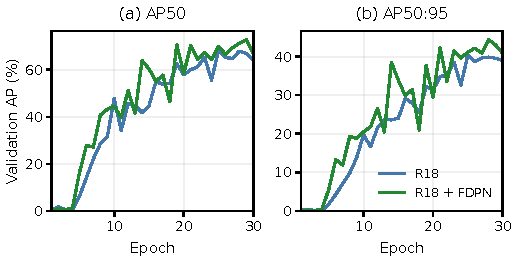
\includegraphics[width=\columnwidth]{initial_penn_curves_column.pdf}
\caption{Initial single-seed Penn--Fudan validation AP over 30 epochs (seed 2026). Curves are descriptive and do not represent seed variability or convergence.}
\label{fig:initial_curves}
\end{figure}

\subsection{Training-Budget Sensitivity}
Table~\ref{tab:budget_sensitivity} retains the signed FDPN-minus-baseline differences under both budgets, including the COCO \mapfifty{} decrease. The 100-epoch extension is exploratory and reuses the 30-epoch test partitions. Differences are calculated before rounding.

\begin{table}[!htbp]
\centering
\caption{Training-budget sensitivity: FDPN minus baseline in percentage points.}
\label{tab:budget_sensitivity}
\footnotesize
\setlength{\tabcolsep}{5pt}
\begin{tabular}{llrr}
\toprule
Dataset & Epochs & $\Delta$AP$_{50}$ & $\Delta$AP$_{50:95}$\\
\midrule
VOC-person & 30 & +9.24 & +3.28\\
VOC-person & 100 & +2.84 & +0.56\\
COCO-person & 30 & -0.61 & +0.16\\
COCO-person & 100 & +2.40 & +1.19\\
\bottomrule
\end{tabular}
\end{table}


\subsection{Three-Seed and Capacity-Control Evaluation}
Each configuration is trained afresh with seeds 2026--2028 on the same partition. CCFF-320 widens only baseline fusion, preserving the backbone, AIFI, and decoder architecture. Width is selected before training by parameter proximity: 22.029 M versus 22.236 M inference parameters, a 0.93\% gap. FLOPs and latency are not matched.

FDPN-minus-baseline \mapcoco{} differences are +1.88, +1.06, and +0.74 points; mean \mapfifty{} decreases by 1.42 points. Against CCFF-320, FDPN is lower for seed 2026 and higher for the others, with a mean advantage of 0.86 points. Table~\ref{tab:robustness} and Fig.~\ref{fig:seed_results} report the summary and individual runs.

Sample standard deviations use denominator $n-1$ with $n=3$. They describe seed variability on a reused 25-image test partition, not uncertainty across datasets or guaranteed equivalence to historical runs.

\section{Implementation Interfaces}
The two FocusFeature instances at layers 11 and 18 have independent parameters and use the fixed kernel set $\{5,7,9,11\}$. Refocusing is a second aggregation, not recurrent weight sharing. The decoder consumes layers 24, 18, and 21, with strides $\{8,16,32\}$ and channels $\{256,576,256\}$. Its input projections adapt these widths to the retained 256-dimensional, three-layer, 300-query decoder. The backbone and AIFI operator structures are retained.

\end{document}
